%%%%%%%%%%%%%%%%%%%%%%%%%%%%%%%%%%%%%%%%%%%%%%%%%%%%%%%%%%%%%%%%%%%%%%%%%%%%%%%%%%%%%%%%%%%%%%%%%%%%%%%
%%%%%%%%%%%%%% Template de Artigo Adaptado para Trabalho de Diplomação do ICEI %%%%%%%%%%%%%%%%%%%%%%%%
%% codificação UTF-8 - Abntex - Latex -  							     %%
%% Autor:    Fábio Leandro Rodrigues Cordeiro  (fabioleandro@pucminas.br)                            %% 
%% Co-autor: Prof. João Paulo Domingos Silva  e Harison da Silva                                     %%
%% Revisores normas NBR (Padrão PUC Minas): Helenice Rego Cunha e Prof. Theldo Cruz                  %%
%% Versão: 1.0     13 de março 2014                                                                  %%
%%%%%%%%%%%%%%%%%%%%%%%%%%%%%%%%%%%%%%%%%%%%%%%%%%%%%%%%%%%%%%%%%%%%%%%%%%%%%%%%%%%%%%%%%%%%%%%%%%%%%%%
\section{\esp Introdução}

Em um mercado globalizado e competitivo, as tecnologias da informação se tornaram fundamentais para o auxílio da gestão das empresas em suas atividades rotineiras e também no suporte a tomadas de decisões e a possibilidade de desenvolvimento de novos negócios, novos modelos de negócio e a modificação dos valores estratégicos das empresas. \cite{audy}.

Visando a adequação às mudanças mercadológicas, organizacionais e a manutenibilidade em relação a concorrência, o investimento em sistemas de informação tem uma grande parcela do orçamento das empresas, buscando o alinhamento da Tecnologia da informação e negócios. \cite{luftman}  
Para atender a essas necessidades, os requisitos de sistemas têm se tornado cada vez mais complexos, voláteis e robustos diante das demandas das organizações. 
As denominadas metodologias ágeis permitem a entrega de  \textit{software} funcionais em ciclos de desenvolvimento mais curtos considerando a velocidade demandada para a sua construção. \cite{sbbrocco} 
          
No entanto as equipes que lidam com a infraestrutura têm a difícil tarefa de implantar um \textit{software} em produção a medida em que são criados ou modificados, pois estes sistemas requerem dependências de componentes externos, como configurações de \textit{hardware}, sistemas operacionais, banco de dados, servidores de aplicação e web e ainda configurações específicas da aplicação. Isto demanda um tempo considerável para a implantação destes sistemas.

Para garantir um processo totalmente ágil e que acompanhe as exigências do negócio da organização é necessário que haja uma integração do desenvolvimento de sistemas e as operações de infraestrutura. Portanto essa abordagem ágil também deve ser seguida pelas equipes de infraestrutura.
O movimento cultural denominado DevOps surgido em meados de 2009, foi influenciado principalmente por metodologias ágeis e computação na nuvem. Ele teve como fundamento a automatização de processos das operações de infraestrutura e a integração entre as equipes de desenvolvimento e operações. \cite{sato}.

A automatização de processos de infraestrutura é uma das premissas do DevOps, utilizando uma abordagem para provisionar e gerenciar recursos de computação como máquinas virtuais, discos de armazenamento, regras de segurança, instalação de \textit{software}, regras de redes e qualquer outro componente de serviço, destinando-se a simplificar significativamente a configuração e o gerenciamento de recursos. Ao tratar a infraestrutura como código, as organizações podem usar as melhores práticas de desenvolvimento de software, incluindo revisão de código e controle de versão, documentação e testes. Esta abordagem reduz a complexidade do gerenciamento,pois, todo o processo e dividindo em tarefas em menores e em mais processos gerenciáveis.A abordagem da infraestrutura como código ou também conhecida como IaC, reduz os riscos operacionais, permitindo revisar o código e salvar todas as revisões anteriores de uma infraestrutura codificada, podendo restaurar a infraestrutura em qualquer revisão anterior quando necessário.

Segundo \citeonline{Morris:2016:ICM:3006361}, a essência da infraestrutura como código é submeter a configuração da infraestrutura da mesma maneira que o código fonte do software é tratado, usando sistemas de gerenciamento de código-fonte, \textit{TDD} \footnote{\textit{TDD - Test Driven Development}: O teste são que são escritos antes do nosso código de produção} , integração contínua \footnote{\textit{CI - Continuous Integration}: É uma prática de desenvolvimento de software em que os desenvolvedores, juntam suas alterações de código em um repositório central e os testes são executados. Geralmente, a integração contínua se refere ao estágio de criação ou integração do processo de lançamento de software  }, refatoração de código e outras técnicas que são úteis para garantir que as alterações na infraestrutura sejam exaustivamente testadas, repetíveis e transparentes.


\section{\esp Metodologia}

\subsubsubsection{Tecnologias utilizadas}


\subsubsubsection{Artefatos produzidos}


\subsubsubsection{Métricas de Validação}


\section{\esp Trabalhos Relacionados} \label{relacionados}


\citeonline{Carnegie} explica que o \textit{design} da infraestrutura é a fase do ciclo de vida do produto em que se define e configura os recursos necessários para o funcionamento dele. A Infraestrutura como código é um conjunto de práticas que usam código para configurar recursos, como máquinas e redes (virtuais), instalar programas, configurar um banco de dados e definir uma regra de segurança. As práticas IaC permitem a criação de vários recursos de maneira automatizada e padronizada, controlando o estado da infraestrutura, além disso permitem o controle de versão, ou seja, pode-se desfazer de qualquer mudança na infraestrutura, somente alterando o código do recursos. Ele também cita que antes mesmo do surgimento da IaC os administradores de sistemas já utilizavam automação, através de \textit{script} para realizar as tarefas de configuração de infraestrutura. E que a IaC surgiu com a popularização da computação da nuvem como serviço e que todos os recursos oferecidos são virtuais. No artigo ele ainda descreve que os provedores de serviços em nuvem fornecem um console de gerenciamento(uma interface \textit{web}) para a administração de recursos. Porém, para um sistema de larga escala, usar o console não é muito prático devido à dificuldade de gerenciar centenas de recursos que são criados e destruídos com uma grande frequência deve-se usar as \textit{application program interface} \footnote{É um conjunto de rotinas e padrões de programação para acesso a um aplicativo de \textit{software} ou plataforma baseada na \textit{Web}, permitindo que dois aplicativos se comuniquem. } (API) disponibilizadas pelo provedor ou Ferramentas IaC  que interagem com essas API que resolvem a questão da criação e destruição de alta frequência desses recursos. Por fim ele cita a relação entre infraestrutura como código \textit{Agile} e o DevOps. 

\hfill

Segundo \citeonline{masek}, a popularização da virtualização e o crescente poder dos servidores e a disponibilidade da computação em nuvem levaram a um aumento significativo no número de servidores e estações de trabalho que precisam ser gerenciados. Nesse ponto, as ferramentas de gerenciamento de orquestração e gerenciamento de configuração se aplicam nesses casos. Os administradores de sistema gerenciam grupos de servidores ou estações de trabalho idênticas (máquinas físicas ou máquinas virtuais) que executam aplicativos e serviços idênticos. Em seu artigo ele apresenta um estudo sobre o uso da ferramenta \textit{Ansible} nos laboratórios da \textit{Brno University of Technology (BUT)}. Ele descreve que o objetivo de utilizar uma ferramenta de IaC é fornecer uma plataforma para gerenciar com eficiência a infraestrutura de larga escala dos laboratórios universitários, com o mínimo de contribuição de desenvolvedores ou administradores.
O autor descreve a infraestrutura como código, como o gerenciamento de redes infraestrutura de trabalho (por exemplo,  em um modelo descritivo. Ele cita dois grupos de ferramentas de infraestrutura como código mais populares: \textit{Chef, Puppet, Ansible e SaltStack}, sendo todas “ferramentas de gerenciamento de configuração”, o que significa que elas foram projetadas para instalar e gerenciar \textit{software} em servidores e estações de trabalho já existentes. E as ferramentas \textit{CloudFormation, Terraform} são “ferramentas de orquestração”, o que significa que eles são projetados para provisionar os servidores.

\hfill

 \citeonline{steve} fala da importância da escolha de ferramentas de IaC como (\textit{ Chef, Ansible, Puppet, SaltStack, Terraform }) se deve levar em consideração o conjunto de casos em que essas ferramentas se propõem a resolver. Estas ferramentas são classificadas em dois domínios: gerenciamento de configurações e orquestração de configuração e quais casos elas resolveram. O autor ainda explica os conceitos de infraestrutura mutável e imutável, escrita de código procedural e declarativa. Este conceitos serão abordados na seção \ref{IaC}. 

\citeonline{steve} expressa que se deve escolher uma ferramenta focada na orquestração de infraestrutura e outra em gerenciamento de configuração de aplicativos reunindo os benefícios de ambas, pois os desafios do gerenciamento de provisionamento e configuração estão intimamente relacionados, porque as organizações geralmente provisionam os servidores e implantam aplicativos neles. E ai que os tipos de ferramentas de IaC vão se convergir.   

\section{\esp IaC ou Infraestrutura como código} \label{IaC}

Os items apresentados neste capítulo foram levantados de acordo com assuntos abordados na seção \ref{relacionados}. A ideia dessa seção é descrever os conceitos básicos da infraestrutura como código de forma sucinta para um entendimento geral do assunto.  

\subsection{Gerenciamento de Configuração} 
Ferramentas de gerenciamento de configuração como \textit{Chef, Puppet, Ansible,Saltack} foram projetadas para instalar e gerenciar softwares em servidores já existentes. Por exemplo podendo instalar um banco de dados, adicionar uma regra de \textit{firewall}, realizar uma atualização no sistema operacional. 

\subsection{Provisionamento}

Ferramentas de Provisionamento como \textit{Terraform, Heat, Cloudformation} foram projetadas criar as próprias instâncias \footnote{Uma instância é um servidor virtual na nuvem. Por exemplo: Uma instância rodando o sistema operacional LINUX} e a inicialização de seus recursos. As ferramentas geralmente se concentram no resultado final e ajudam a garantir que o ambiente esteja sempre nesse "estado" 

Segundo \citeonline{Carnegie}, existem sobreposições e esses termos não são mutuamente exclusivos para ambas as ferramentas. As ferramentas de provisionamento podem realizar tarefas de configuração e ferramentas de configuração podem realizar tarefas de provisionamento, porém elas se concentram naquilo que são melhores. 


\subsection{Linguagem}

As ferramentas de IaC usam arquivos de definição como \textit{DSL} 
  \footnote{\textit{DSL - Domain-Specific Language:} Uma linguagem de domínio específico é criada especificamente para resolver problemas em um domínio particular e não se destina a ser capaz de resolver os problemas fora de seu âmbito. }, ou formatos de texto conhecidos comuns como \textit{ YAML} \footnote{\textit{YAML - Ain't  Markup Language}: É um formato de serialização (codificação de dados) de dados legíveis por humanos -  https://yaml.org/ }, \textit{JSON} \footnote{\textit{JSON - JavaScript Object Notation:} É uma formatação leve de troca de dados. Para seres humanos, é fácil de ler e escrever. Para máquinas, é fácil de interpretar e gerar. Está baseado em um subconjunto da linguagem de programação JavaScript, https://www.json.org/json-pt.html}, \textit{XML} \footnote{\textit{XML - eXtensible Markup Language:} é uma linguagem de marcação para a criação de documentos com dados organizados hierarquicamente, tais como textos, banco de dados ou desenhos vetoriais.}
  ou linguagens de programação como \textit{Python} \footnote{\textit{Python} é uma linguagem de programação de alto nível, interpretada, de script, imperativa, orientada a objetos, funcional, de tipagem dinâmica e forte.}  \textit{Ruby} \footnote{\textit{Ruby} é uma linguagem de programação interpretada multi-paradigma, de tipagem dinâmica e forte, com gerenciamento de memória automático.}  ou uma mesclagem de ambas.
 
   \subsubsubsection{Declarativa}
  É o estilo em que você escreve um código que especifica o estado final desejado, e a própria ferramenta IaC é responsável por descobrir como atingir esse estado. Veja o exemplo na Figura \ref{fig:figura2}.
 
 \begin{figure}[ht]
	\centering	
	\caption[\hspace{0.1cm}Exemplo declarativo]{Exemplo de escrita declarativa da ferramenta Terraform}
	\vspace{-0.4cm}
	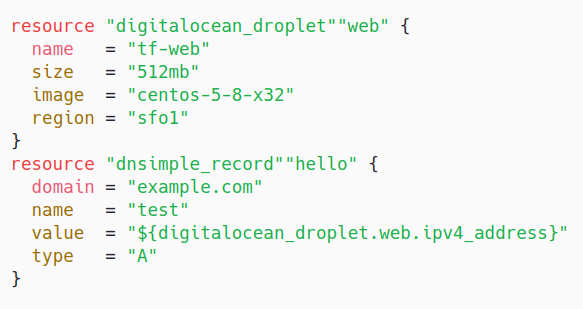
\includegraphics[width=0.98\textwidth]{artigo/figuras/terraform-declarative-exemple-01.png}
	 \vspace{-0.2cm}
	\\\textbf{\footnotesize Fonte: \cite{terraform01} }
	\label{fig:figura2}
\end{figure}
\vspace{-0.5cm}
 
 \subsubsubsection{Procedural}
  
  É o estilo na qual você escreve um código e especifica, passo a passo, como atingir o estado final desejado. O ônus recai sobre o usuário para determinar o processo de implantação ideal. Veja o exemplo na Figura \ref{fig:figura1}.

\begin{figure}[ht]
	\centering	
	\caption[\hspace{0.1cm}Exemplo procedural]{Exemplo de escrita procedural da ferramenta Chef}
	\vspace{-0.4cm}
	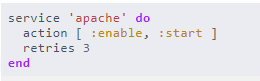
\includegraphics[width=0.5\textwidth]{figuras/chef-io-exemplo-procedural.png}
	 \vspace{-0.2cm}
	\\\textbf{\footnotesize Fonte: \cite{chef01}}
	\label{fig:figura1}
\end{figure}
\vspace{-0.5cm}
  

 \subsection{Infraestrutura}
 
 \subsubsubsection{Mutável}
 Na infraestrutura mutável uma mudança de software será executada nos servidores existentes e com o tempo, à medida em que atualizações são realizadas, cada servidor tem um histórico único de alterações levando erros sutis de configuração. As ferramentas de gerenciamento de configuração, normalmente são padronizadas para um paradigma de infraestrutura mutável.
 
  Um exemplo: Digamos o JAVA precisa ser atualizado. Na infraestrutura mutável cada servidor precisa atualizar a versão do JAVA, geralmente esta atualização pode ser desempenhada por uma ferramenta de gerenciamento de configuração. 
 
 \subsubsubsection{Imutável}
  Segundo \citeonline{Dadgar} A Noção de imutabilidade é a ideia de que, uma vez criada uma coisa, não a mudamos após a criação.
 
 Na infraestrutura imutável qualquer alteração a ser realizada nos servidores eles devem ser recriados. Estas alterações são feitas criando novas configurações e novos servidores são criados a partir delas. Isso aumenta a previsibilidade porque este servidor já foi testado antes de ir para a produção. Em outras palavras, as implantações se tornam atômicas. As ferramentas de provisionamento desempenham este papel.\cite{Morris:2016:ICM:3006361}.
 
 Um exemplo: Digamos que precisamos atualizar o \textit{JAVA}\footnote{Java é uma linguagem de programação e plataforma computacional.} para uma versão mais nova. Na infraestrutura imutável é criado um novo servidor com essa atualização. Esta configuração é testada então novos servidores são criados a partir desta configuração e todos que estão rodando a versão antiga do java serão destruídos. 
 
\subsection{Arquitetura}

\subsubsubsection{Cliente ou Masterless} \label{semagent}
Segundo \citeonline{Jan-Piet} conforme citado por \citeonline{Morris:2016:ICM:3006361} na arquitetura cliente não existe um servidor central e não é necessário instalar agentes nos nós gerenciados. 
o que torna a configuração mais simples. A configuração é feita escolhendo uma máquina e instalando o cliente e informando os IP's \footnote{\textit{Internet Protocol}} dos nós ele deve gerenciar no arquivo de configuração do programa. A autenticação é realizada por meio do protocolo \textit{SSH} \footnote{\textit{SSH - Sever Secure Shell:}  É um protocolo de rede criptográfico para operação de serviços de rede de forma segura sobre uma rede insegura. Baseado na arquitetura cliente-servidor, ele conecta uma aplicação cliente \textit{SSH} com um servidor \textit{SSH}, permitindo a execução remota de comandos.} , Ao alterar algum recurso ele se conecta ao no \textit{IP} e executa as alterações. Veja a Figura \ref{fig:figura3}. 

Exemplo de ferramentas: \textit{Ansible}

\begin{figure}[ht]
	\centering	
	\caption[\hspace{0.1cm}Exemplo arquitetura Cliente]{Exemplo geral de arquitetura Cliente}
	\vspace{-0.4cm}
	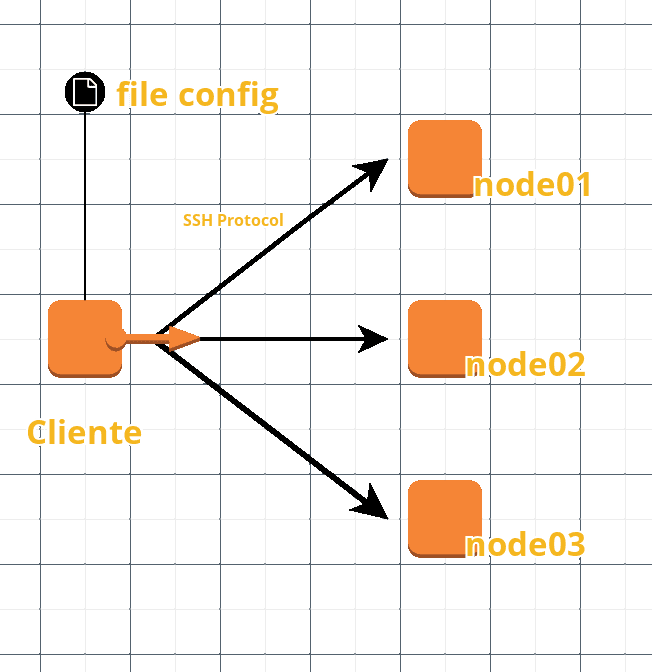
\includegraphics[width=0.5\textwidth]{figuras/cliente.png}
	 \vspace{-0.2cm}
	\\\textbf{\footnotesize Fonte: Próprio Autor}
	\label{fig:figura3}
\end{figure}
\vspace{-0.5cm}


As ferramentas de provisionamento se comunicam diretamente com a \textit{API} do provedor de serviços de nuvem \footnote{Um provedor de serviços de nuvem é uma empresa contratada que fornece uma plataforma, infraestrutura, aplicativo ou serviços de armazenamento baseados em nuvem. Em que você paga conforme o uso. Por exemplo: \textit{Amazon Web Service, Azure, Digital Ocean, Google Cloud.}. Eles também são conhecido pelo termo \textit{IaaS - Infrastructure as a service} }

Exemplo de ferramentas: \textit{Terraform}

\subsubsubsection{Mestre/Agente ou Cliente/Servidor} \label{cliente-servidor}
 
 Segundo a \citeonline{puppetlabs}, nessa arquitetura (Figura \ref{fig:figura4}), um servidor \footnote{Dependendo da ferramenta o \textit{master} pode ser representado por mais de um servidor} central denominado mestre controla as informações de configuração de cada nó(cada servidor tem instalado e um agente, geralmente rodando como um processo em segundo plano \footnote{Processos em que não há interação com o usuário}). Este agente solicita seu próprio catálogo de configuração ao mestre.  
 
 Periodicamente, cada agente envia informações ao mestre e solicita um catálogo. O mestre compila e retorna o catálogo de alterações desse nó, usando várias fontes de informações às quais ele tem acesso. Ao receber este catálogo com as alterações a serem realizadas o agente aplica as alterações no nó. 
 
 Em outras palavras o fluxo básico de funcionamento é: Quando se altera as definições de um recurso, por exemplo, uma nova versão do \textit{Apache} \footnote{É um servidor \textit{web}, compatível com o protocolo HTTP, mantido pela \textit{Apache Software Foundation }}, estas são submetidas para o mestre. Quando o Agente solicita informações do mestre, o mestre compila e retorna o catálogo com as alterações para o nó desse agente usando as fontes de informação às quais o mestre tem acesso, o agente recebe essas alterações então ele aplica nó correspondente, alterado a versão do \textit{Apache}.   

Essa arquitetura pode ter uma leve variação entre ferramentas podendo ter uma máquina de onde é acessado o mestre para que depois sejam replicadas nos nó.

Embora essas ferramentes podem ser usada para o gerenciamento de estações de trabalho não é o objetivo deste estudo.

Exemplo de ferramentas: \textit{Puppet,Chef} 

 \begin{figure}[ht]
	\centering	
	\caption[\hspace{0.1cm}Exemplo arquitetura Master/Agent]{Exemplo geral de arquitetura Master/Agent}
	\vspace{-0.4cm}
	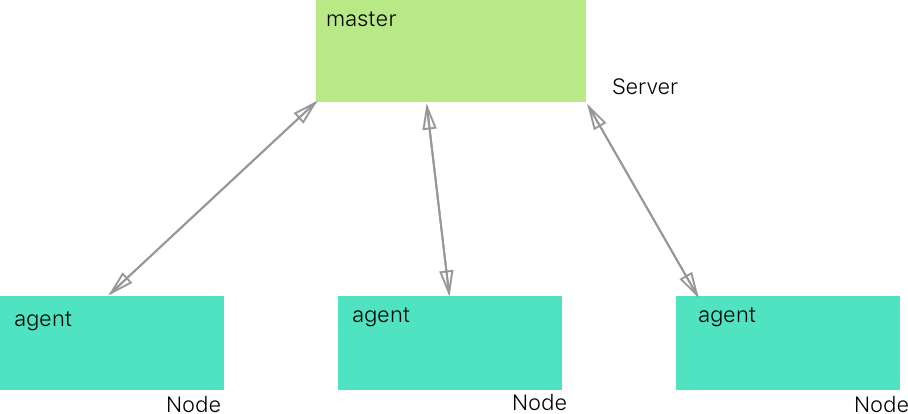
\includegraphics[width=0.5\textwidth]{figuras/master-agent.png}
	 \vspace{-0.2cm}
	\\\textbf{\footnotesize Fonte: \cite{Harit}}
	\label{fig:figura4}
\end{figure}
\vspace{-0.5cm}

\section{Ferramentas}

Esta seção aborda os principais conceitos das ferramentas utilizada neste artigo e as definições destes conceitos foram retiras diretamente da documentação oficial das ferramentas que podem ser consultadas respectivamente aqui: 

\href{https://docs.ansible.com}{https://docs.ansible.com} e \href{https://terraform.io/docs}{https://terraform.io/docs}

\textit{Ansible} e \textit{Terraform} operam usando uma arquitetura sem agente(conforme mencionado no item \ref{semagent}) e promovem uma interface simplificada legível para a definição de recursos, facilitando a adoção. As definições de conceitos foram retirados diretamente da documentação oficial das ferramentas.


\subsubsubsection{Ansible}

\textit{Ansible} é uma suíte completa de automação de processos de TI radicalmente simples, ela abrange desde o provisionamento e o gerenciamento de configurações e outras necessidades..

Ele não usa agentes e nenhuma infraestrutura de segurança personalizada adicional(uma características de ferramentas, conforme mencionado no item \ref{cliente-servidor}), por isso é relativamente fácil de implantar. O \textit{Ansible} usa uma linguagem muito simples a \textit{YAML} na forma que eles descrevem como \textit{Ansible Playbooks} que permite descrever seus trabalhos de automação de uma maneira que se aproxima do inglês. 

Ele é descentralizado e depende de das credenciais do sistema operacional existentes para controlar o acesso a máquinas remotas. A principal e mais usada forma dele se conectar é usando o protocolo \textit{SSH}.Se necessário, ele pode se conectar facilmente por \textit{Kerberos} \footnote{É um protocolo desenvolvido para fornecer poderosa autenticação em aplicações usuário/servidor, onde ele funciona como a terceira parte neste processo, oferendo autenticação ao usuário.}, \textit{LDAP} \footnote{\textit{LDAP - Lightweight Directory Access:} É um protocolo de aplicação aberto para acessar e manter serviços de informação de diretório distribuído sobre uma rede de IP, permitindo o compartilhamento de informações sobre usuários, sistemas, redes, serviços e aplicações através da rede.} e outros sistemas de gerenciamento de autenticação centralizados.


\textit{Ansible} nasceu como uma ferramenta de gerenciamento de configurações e a partir da versão 2.0 passou a ser uma suíte completa e também podendo provisionar infraestrutura neste artigo abordaremos apenas como uma ferramenta de configuração o que ainda ele é muito citado na literatura como essas características.

 O \textit{Ansible} apresenta os seguintes itens em sua arquitetura:

\hfill

\textbf{\textit{Controller Machine}}: É máquina de onde o \textit{Ansible} está sendo executado. 

\textbf{\textit{Modules}}: Um módulo normalmente abstrai uma tarefa do sistema, por exemplo instalar um determinado aplicativo e configurar, para não ficar reescrevendo esta tarefa quando precisar, um módulo pode ser escrito para isso e usando qualquer linguagem de programação. Então bastando referenciar este módulo em alguma tarefa. O \textit{Ansible} se conecta aos seus nós(máquinas) e envia os chamados e executa esses módulos (por \textit{SSH} por padrão) e os remove quando finalizados.   

\textbf{\textit{Plugins}}: Os \textit{plugins} oferecem uma extensões para os principais recursos do \textit{Ansible}, por exemplo um \textit{plugin} para envio de \textit{e-mail}. Um \textit{plugins} deve ser escritos em \textit{Python}. Diferente dos módulos os \textit{plugins} são executados na máquina de controle.

\textbf{\textit{Inventory}}: É um arquivo de configuração que contém informações sobre os servidores os nós(servidores) que ele esta gerenciando. Todo o servidor gerenciado deve ser informado nesse arquivo.

\textbf{\textit{Playbooks}}: É principal item é o ponto de entrada para definir os recursos, escritos por meio do formato \textit{YAML}.

\textbf{\textit{Role}}: Uma maneira predefinida de organizar \textit{playbooks} e outros arquivos para facilitar o compartilhamento e a reutilização.

\textbf{\textit{Play}}: Uma execução de um \textit{playbook} do início ao fim.

\textbf{\textit{Facts}}: Variáveis globais que contêm informações sobre o sistema, como interfaces de rede ou sistema operacional.

\textbf{\textit{Task}}: Um bloco de código que define um único procedimento a ser executado, por exemplo, instalar o \textit{Apache}.

 \begin{figure}[ht]
	\centering	
	\caption[\hspace{0.1cm}Exemplo de funcionameno do Ansible]{Exemplo de funcionameno do Ansible}
	\vspace{-0.4cm}
	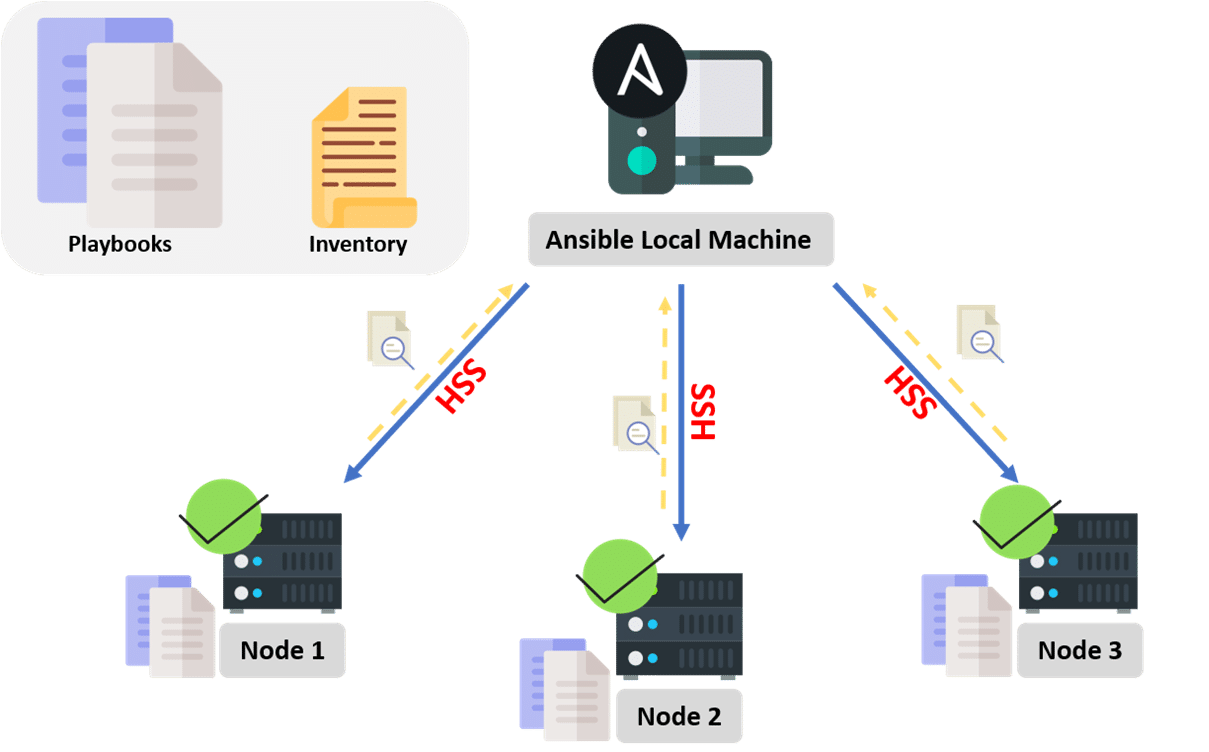
\includegraphics[width=0.5\textwidth]{figuras/ansible-working.png}
	 \vspace{-0.2cm}
	\\\textbf{\footnotesize Fonte: \cite{intellipaat}}
	\label{fig:figura6}
\end{figure}
\vspace{-0.5cm}

\subsubsubsection{Terraform} 

 O \textit{Terraform} é uma ferramenta para provisionamento de infraestrutura, permite criar, alterar e criar versões de infraestrutura com segurança e eficiência. Ele pode gerenciar os mais populares provedores de nuvem e também trabalhar com soluções internas personalizadas.

O \textit{Terraform} usa uma linguagem \textit{DSL} muito simples a \textit{HCL} \footnote{\textit{HCL - Hashicorp Configuration Language.} Veja mais em: \href{https://www.terraform.io/docs/configuration/syntax.html}{https://www.terraform.io/docs/configuration/syntax.html} } (veja na Figura \ref{fig:figura2}.) com a extensão de arquivo \textit{"*.tf"} para a definição de recursos de infraestrutura. 

Os arquivos de configuração descrevem para o \textit{Terraform} os componentes necessários para criar um único aplicativo ou toda a configuração da infraestrutura. Ao executar ele gera um plano de execução descrevendo o que fará para atingir o estado desejado e, em seguida, executa-o para construir a infraestrutura descrita. 
À medida que a configuração muda, ele determina o que mudou e criar planos de execução incrementais para serem aplicados.

Uma característica do \textit{Terraform} é garantir que ao executar um arquivo de definição de recursos varias vezes o resultado será o mesmo, ou seja a \textbf{idempotência} \footnote{É a propriedade que algumas operações têm de poderem ser aplicadas várias vezes sem que o valor do resultado se altere após a aplicação inicial.} de uma operação.

O \textit{Terraform} pode criar e gerenciar componentes de baixo nível como instâncias de servidores, armazenamento e componentes de alto nível(Aqui o \textit{Terraform} se sobrepõem com ferramentas de gerenciamento de configuração), como configurar um \textit{DNS} \footnote{\textit{DNS -Domain Name System}: É responsável por localizar e traduzir para números IP os endereços dos sites que digitamos nos navegadores.} de uma máquina.

Além disso o terraform o terraform pode ser integrado com a ferramentas de gerenciamento de configuração, como \textit{Ansible, Chef ou Puppet}

Os principais conceitos dele são:

\textbf{Infraestrutura como código}: A infraestrutura é descrita usando uma sintaxe de configuração de alto nível. Isso permite que os recursos da infraestrutura sejam versionados e tratado como qualquer outro código. Além disso, a infraestrutura pode ser compartilhada e reutilizada.

\textbf{Planos de Execução}: O \textit{Terraform} possui uma etapa de "planejamento" onde gera um plano de execução . O plano de execução mostra o que o \textit{Terraform} fará quando você chama aplicar. Isso permite evitar surpresas quando o ele manipula a infraestrutura.

\textbf{Gráfico de Recursos}: Ele cria um gráfico de todos os recursos e paralela a criação e modificação de quaisquer recursos não dependentes. Por esse motivo, o \textit{Terraform} constrói a infraestrutura da maneira mais eficiente possível, e os operadores obtêm entendimento sobre as dependências dos recursos.

\textbf{Automação de Mudanças}: Conjuntos de alterações complexas podem ser aplicados à infraestrutura com mínimo de interação humana. Com o plano de execução e o gráfico de recursos, permite sabe exatamente o que o \textit{Terraform} mudará e em que ordem, evitando muitos possíveis erros humanos.

\textbf{Estado da infraestrutura}: É um registro dos recursos provisionados no momento e que guardam o estado da infraestrutura e ativam o histórico das alterações incrementais. O estado pode ser armazenado remotamente e localmente. O armazenamento de estado remoto permitem que as equipes compartilhem o estado, evitem mais de uma alteração por vez e visualizem um histórico de todas as alterações na infraestrutura por equipe.

\textbf{\textit{Providers}}: Um provedor é responsável por entender as interações da \textit{API} e expor os recursos. Os provedores geralmente são serviços de \textit{IaaS},  por exemplo : \textit{Amazon
Web Service, Azure, Digital Ocean, Google Cloud, DNSimple, CloudFlare, Digital Ocean}).

\textbf{\textit{Resource}}: Um recurso fornecido por um provedor, por exemplo: Uma instância, Um disco   

\textbf{\textit{Provisioners}}: Os provisionadores podem ser usados para executar ações específicas na máquina local ou remota, por exemplo: copiar um arquivo da máquina local para a máquina remota.

\textbf{\textit{Modules}}: Um módulo é um agrupamento para vários recursos que são usados juntos. Os módulos podem ser usados para criar abstrações leves, para que você possa descrever sua infraestrutura em termos de arquitetura, em vez de diretamente em termos de objetos físicos.

\textbf{\textit{Variables}}: Usando um espaço reservado especial para inserir um valor calculado em uma sequência de caracteres. 

 \textbf{\textit{Variables output}}: Dados exportados por um módulo, que podem ser exibidos para um usuário e  ou usados de forma programática por outro código \textit{Terraform}.
 
 \textbf{\textit{Plugins}}: O \textit{Terraform} é construído em uma arquitetura baseada em \textit{plugins}. Todos os provedores e provisionadores usados nas configurações do \textit{Terraform} são \textit{plugins}. Os usuários do \textit{Terraform} podem escrever novos \textit{plugins} para oferecer suporte a novas funcionalidades no \textit{Terraform}.
 
  \begin{figure}[ht]
	\centering	
	\caption[\hspace{0.1cm}Exemplo de funcionamento do Terraform]{Exemplo de funcionamento do Terraform}
	\vspace{-0.4cm}
	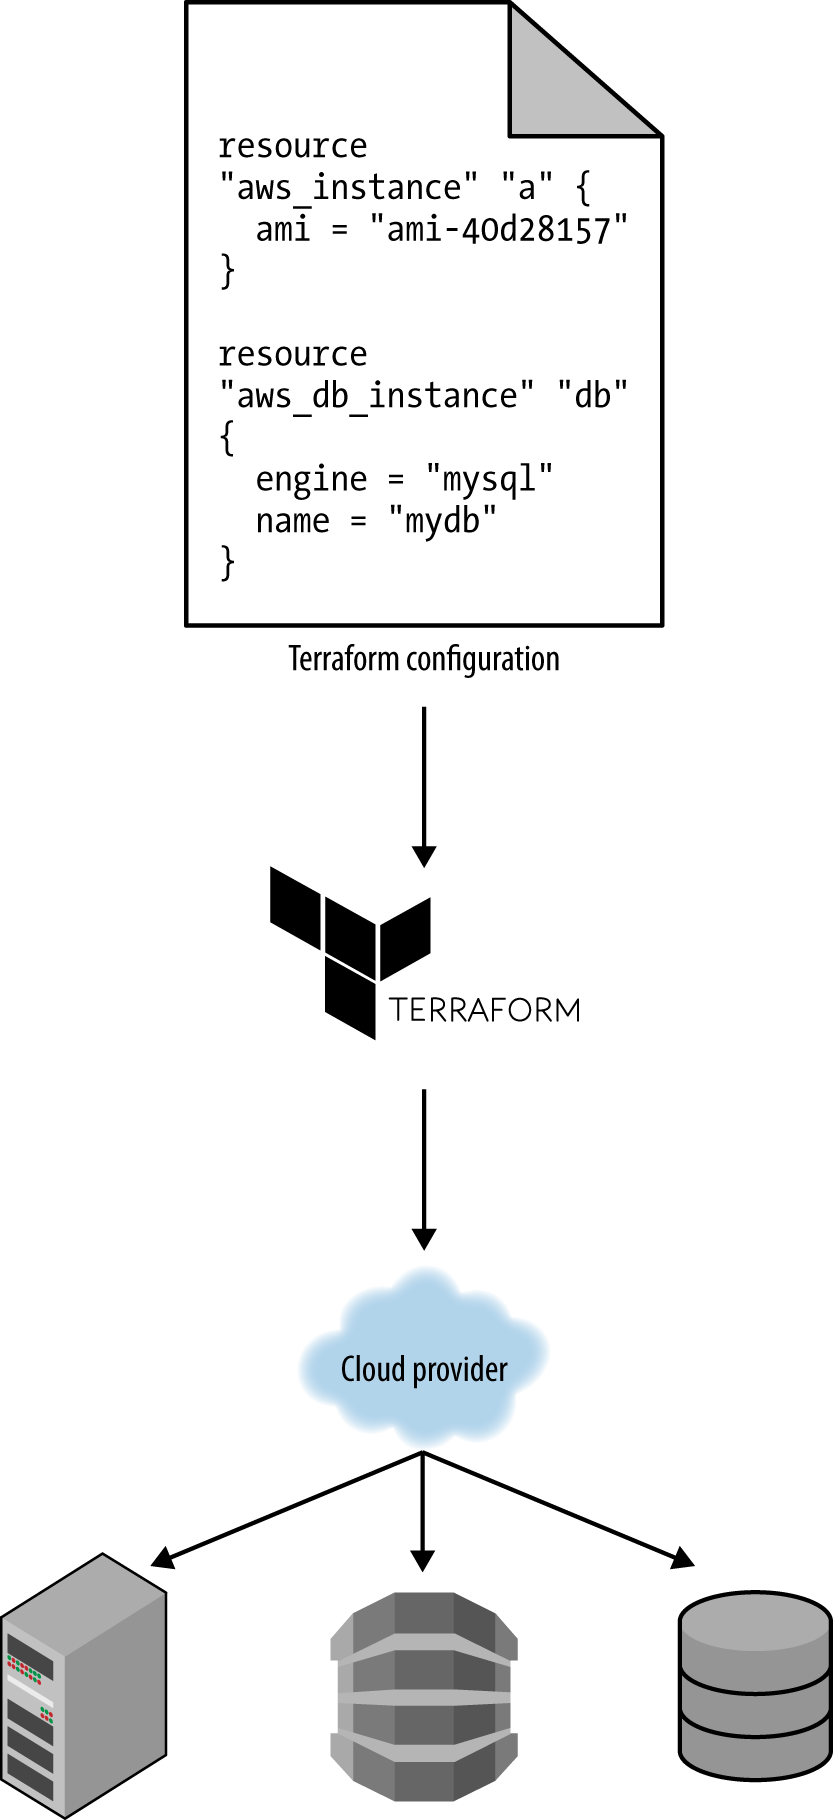
\includegraphics[width=0.5\textwidth]{figuras/terraform-working.png}
	 \vspace{-0.2cm}
	\\\textbf{\footnotesize Fonte: \cite{oreilly}}
	\label{fig:figura7}
\end{figure}
\vspace{-0.5cm}

\subsection{Ferramentas Auxiliares}

\textbf{\textit{Gitbub}} é uma plataforma baseada em \textit{VCS - Version Control System} que registra as mudanças feitas em um arquivo ou um conjunto de arquivos ao longo do tempo de forma que possa recuperar versões específicas. 

\textbf{\textit{Azure}}: O \textit{Microsoft Azure} é um conjunto serviços de nuvem que permite criar, gerenciar e implantar aplicativos em uma enorme rede global. 

\textbf{\textit{Azure Pipelines}}: É uma ferramenta de integração contínua e entrega contínua baseado em nuvem.



 